\documentclass{article}
\usepackage[utf8]{inputenc}
\usepackage{fancyhdr}
\usepackage{float}
\usepackage{graphicx}
\usepackage{tabularx}
\usepackage{makecell}
\usepackage{multirow}
\usepackage{changepage}

\graphicspath{ {./img/} }

\pagestyle{fancy}  
\setlength\parindent{0pt}
\renewcommand\headrulewidth{0.4pt}                                      
\renewcommand\footrulewidth{0.4pt}
\setlength{\footskip}{60pt}

\title{SE 4GB6: Hazard Analysis\\The Cut}
\author{Group 17\\\\
            Joseph Lu - luy89 \\
            Matthew Po - pom \\
            Stanley Liu  liuz23 \\
            Suhavi Sandhu - sandhs11
            }
\date{\today}

% Setup fancyhdr package
\fancyhf{}
\fancyhfoffset{0em}
% Remove head rule
\renewcommand{\headrulewidth}{0pt}
\renewcommand{\footrulewidth}{0pt}
\fancyfoot[L]{Group17 - The Cut}
\fancyfoot[C]{Page \thepage}
\fancyfoot[R]{Revision 0}

\begin{document}

\maketitle
\newpage
\tableofcontents
\listoffigures
\listoftables
\newpage

\section{Revisions}
\begin{table}[H]
    \caption{Revision}
    \centering
    \begin{tabularx}{\textwidth}{|c|c|c|X|}
        \hline
        Date & Revision Number & Authors & Comments \\ 
        \hline
        January 15, 2020 & 0 & \makecell{Matthew Po\\Suhavi Sandhu\\Stanley Liu\\Joseph Lu} & -\\ 
        \hline
    \end{tabularx}
    \label{tab:Revision}
\end{table}

\newpage

\section{Introduction}

\subsection{Document Purpose}

In this document we will highlight the possible hazards to the success of our project. A hazard is characterized as a scenario that can potentially cause the system to fail. We will also be discussing ways in which we can mitigate each hazard.

\subsection{Scope}

The scope of the project is to be able to identify movies from short video clips. The development team will be focusing on Hollywood movies. Users will be able to input a video clip and the system will give a list of movies with confidence percentages. The scope of the information that will be retrieved is meta data such as actors, release date and description.

\subsection{Definitions}

\begin{table}[H]
    \centering
    \begin{tabular}{|c|c|} 
        \hline
         Catastrophic Failure & The system is unable to process any requests.\\ \hline
    \end{tabular}
    \caption{Definitions}
    \label{tab:Definitions}
\end{table}

\section{Component Overview}

\subsection{Context Diagram of Components}

\begin{figure}[H]
    \centering
    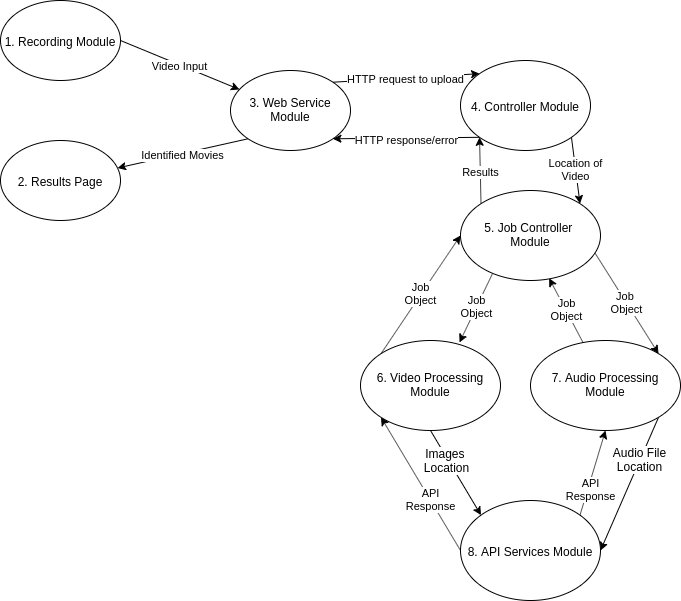
\includegraphics[width = 15cm]{img/ComponentDiagram.png}
    \caption{Context Diagram Showing Boundaries}
    \label{fig:Context}
\end{figure}

\subsection{Module Description}

\renewcommand{\labelenumi}{\Alph{enumi}}
\begin{enumerate}
    \item \textbf{Recording Module}: The user will interact with this module in order to record a video.
    \item \textbf{Web Service Module}: This module will handle communication between the client and server side, such as uploading the video to a dedicated server space.
    \item \textbf{JobController Module}: This module will route jobs to modules when necessary.
    \item \textbf{Video Processing Module}: This module will handle the way the visual portion of the input is analyzed.
    \item \textbf{Audio Processing Module}: This module will handle the way the auditory portion of the input is analyzed.
    \item \textbf{API Services Module}: This module will communicate with third-party APIs such as Google Cloud Vision.
    \item \textbf{Controller Module}: This module will manage communication in the server and is responsible for sending errors and final results back to the user
\end{enumerate}

\section{Software Hazards}
\renewcommand\thesubsection{\thesection.\Alph{subsection}}

\subsection{Recording Module}
\renewcommand{\labelenumi}{\arabic{enumi}}
\begin{enumerate}
    \item User does not give the application permission to access camera on device
\end{enumerate}

\subsection{Web Service Module}
\begin{enumerate}
    \item Failure to establish a connection with the web server to transfer video file
    \item Incomplete transfer of video to server
\end{enumerate}

\subsection{Job Controller Module}
\begin{enumerate}
    \item Corrupt video file detected (Invalid/Cannot find video file/location)
    \item Failure to create new job object (threading issue)
\end{enumerate}

\subsection{Video Processing Module}
\begin{enumerate}
    \item Failure to split images from video
\end{enumerate}

\subsection{Audio Processing Module}
\begin{enumerate}
    \item Failure to parse audio from video
\end{enumerate}

\subsection{API Service Module}
\begin{enumerate}
    \item Failure to establish connection with third party APIs
\end{enumerate}

\subsection{Controller Module} 
\begin{enumerate}
    \item Unable to process client requests
\end{enumerate}

\section{Correlation between Hazard Functions\\and Requirements}
\renewcommand\thesubsection{\thesection.\arabic{subsection}}

\begin{table}[H]
    \centering
    \begin{tabular}{|c|c|} \hline
        \textbf{Hazard Function} & \textbf{Functional and Non-Functional Requirement} \\ \hline
        \multirow{2}{*}{A1: User does not give the application} & F1\\ \cline{2-2}
         & F2\\ \hline
    \end{tabular}
    \caption{Correlation between Hazard Function A1 and Requirements}
    \label{tab:A1Req}
\end{table}

\begin{table}[H]
    \centering
    \begin{tabular}{|p{0.3\textwidth}|c|} \hline
        \textbf{Hazard Function} & \textbf{Functional and Non-Functional Requirement} \\ \hline
        \multirow{6}{0.3\textwidth}{B1: Failure to establish a connection with web server to transfer video file} & F1\\ \cline{2-2}
         & F2\\ \cline{2-2}
         & NF7\\ \cline{2-2}
         & NF9\\ \cline{2-2}
         & NF10\\ \cline{2-2}
         & NF11\\ \hline
    \end{tabular}
    \caption{Correlation between Hazard Function B1 and Requirements}
    \label{tab:B1Req}
\end{table}

\begin{table}[H]
    \centering
    \begin{tabular}{|c|c|} \hline
        \textbf{Hazard Function} & \textbf{Functional and Non-Functional Requirement} \\ \hline
        \multirow{4}{*}{B2: Incomplete transfer of video file to server} & F3\\ \cline{2-2}
         & F4\\ \cline{2-2}
         & F5\\ \cline{2-2}
         & NF9\\ \hline
    \end{tabular}
    \caption{Correlation between Hazard Function B2 and Requirements}
    \label{tab:B2Req}
\end{table}

\begin{table}[H]
    \centering
    \begin{tabular}{|c|c|} \hline
        \textbf{Hazard Function} & \textbf{Functional and Non-Functional Requirement} \\ \hline
        \multirow{4}{*}{C1: Corrupt video file detected} & F3\\ \cline{2-2}
         & F4\\ \cline{2-2}
         & NF10\\ \cline{2-2}
         & NF11\\ \hline
    \end{tabular}
    \caption{Correlation between Hazard Function C1 and Requirements}
    \label{tab:C1Req}
\end{table}

\begin{table}[H]
    \centering
    \begin{tabular}{|c|c|} \hline
        \textbf{Hazard Function} & \textbf{Functional and Non-Functional Requirement} \\ \hline
        \multirow{4}{*}{C2: Failure to create new job object} & F3\\ \cline{2-2}
         &  F5\\ \cline{2-2}
         &  NF10\\ \cline{2-2}
         &  NF11\\ \hline
    \end{tabular}
    \caption{Correlation between Hazard Function C2 and Requirements}
    \label{tab:C2Req}
\end{table}

\begin{table}[H]
    \centering
    \begin{tabular}{|c|c|} \hline
        \textbf{Hazard Function} & \textbf{Functional and Non-Functional Requirement} \\ \hline
        \multirow{2}{0.5\textwidth}{F1: Failure to establish connection with third party APIs
} & F3\\ \cline{2-2}
         &  F5\\ \cline{2-2}
         &  NF10\\ \cline{2-2}
         &  NF11\\ \hline
    \end{tabular}
    \caption{Correlation between Hazard Function F1 and Requirements}
    \label{tab:F1Req}
\end{table}

\begin{table}[H]
    \centering
    \begin{tabular}{|c|c|} \hline
        \textbf{Hazard Function} & \textbf{Functional and Non-Functional Requirement} \\ \hline
        \multirow{6}{0.5\textwidth}{G1: Failure to establish connection with client service modules} & F5\\ \cline{2-2}
         & NF5\\ \cline{2-2}
         & NF7\\ \cline{2-2}
         & NF9\\ \cline{2-2}
         & NF10\\ \cline{2-2}
         & NF11\\ \hline
    \end{tabular}
    \caption{Correlation between Hazard Function G1 and Requirements}
    \label{tab:G1Req}
\end{table}

\section{FMEA Worksheet}

\subsection{Hazards Considered Out of Scope}
\begin{itemize}
    % Recording Module
    \item Subpar Recording device quality
    \item User records at a poor viewing angle
    \item User records in a dimly lit environment
    \item User records video clip that is $<$ 10 seconds or $>$ 60 seconds.
    % Web Service Module
    \item Interrupt transfer of video file to server
    \item Slow transfer of video file to server
    % Job Controller Module
    \item Corrupt video file detected
    \item Invalid/cannot find video file/location
    \item Failure to create new job object
    % Video Processing Module
    \item Unable to properly process frame images due to poor lighting
    % Audio Processing Module
    \item Unable to properly process sound from video file due to audio interference
    % API Service Module
    \item Failure to establish connection with third party APIs
    % Controller Module
    \item Failure to establish connection with client service modules
\end{itemize}

\subsection{Failure Modes and Effect Analysis Table}
\begin{table}[H]
    \centering
    \begin{adjustwidth}{-\oddsidemargin}{}
    \begin{tabularx}{1.45\textwidth}{|c|c|X|X|X|X|} \hline
       \textbf{Comp}  & \textbf{Hazard} & \textbf{Hazard Causes} & \textbf{Hazard Effect} & \textbf{Hazard Detection} & \textbf{Recommended Action} \\ \hline
        A & 1 & User does not give permission to the application to access the camera on the device & Unable to record video & Software check during startup of application & Prompt user to give access to camera during startup of application \\ \hline
        B & 1 & Poor connection from client device & Unable to upload video to web server & Software check for HTTP response codes & Prompt user to re-upload when they have established a secure connection \\ \hline
        B & 1 & Hosting platform may be temporarily unavailable & Unable to receive video file from clients & Software check for HTTP response codes & Investigate and repair unreachable server endpoint \\ \hline
        B & 2 & Network connection timeout or server unreachable & Incomplete video transferred or failure to transfer & Software check for HTTP response codes & Prompt user to reupload when they have established a secure connection \\ \hline
        C & 1 & Insufficient memory on server to save video file & Unable to access video file for processing & Software check for valid file location on server filesystem & Remove old / unused video files from filesystem OR establish “expiry” date on saved files to allow for cleanup of filesystem to free up memory space \\ \hline
        C & 2 & System issue while attempting to create asynchronous jobs & Catastrophic failure of system. Unable to establish new jobs for asynchronous processing & Software check & Re-attempt to create asynchronous job with timeout. If timeout limit is reached, further investigation by development team may be required and will result in server system downtime. \\ \hline
        F & 1 & API service temporarily unavailable & Unable to generate results & Software check for HTTP response codes & Investigate and repair unreachable API endpoint. \\ \hline
        F & 1 & Application cannot access API (security key expired) & Unable to generate results & Software check for HTTP response codes & Investigate and repair unreachable API endpoint.\\ \hline
        G & 1 & Server temporarily unavailable & Unable to return results to clients & Server health check & Output error to user. Investigate and repair. \\ \hline
    \end{tabularx}
    \caption{FMEA Table}
    \label{tab:FMEA}
    \end{adjustwidth}
\end{table}

\end{document}
